\scanpage{78}
% archive foliation: 77
\[
\rho_0=
\]
\diagram{\begin{tikzcd}[ampersand replacement=\&,column sep=small,row sep=large]
\&\&E^+\arrow[dddll]\arrow[dddrr]\arrow[d]\arrow[ddl,"\pi_2^+"']\arrow[ddr,"\pi_1^+"]\arrow[ddd,"\pi_0^+" near start]\&\&\\
\&\&\deleted{\unsure{D_{02}}}\,D_{12}\arrow[ddll,dash]\arrow[ddrr,dash]\&\&\\
\&\bullet\,S_2\&\&\bullet\,S_1\&\\
D_{20}\arrow[rrrr,dash]\&\&\bullet\,S_0\&\&D_{01}\\
\&\&E^-\arrow[uul,"\pi_2^-"']\arrow[uur,"\pi_1^-"]\arrow[u,"\pi_0^-"']\arrow[uuu]\arrow[ull,dash]\arrow[urr,dash]\&\&
\end{tikzcd}}

\figure{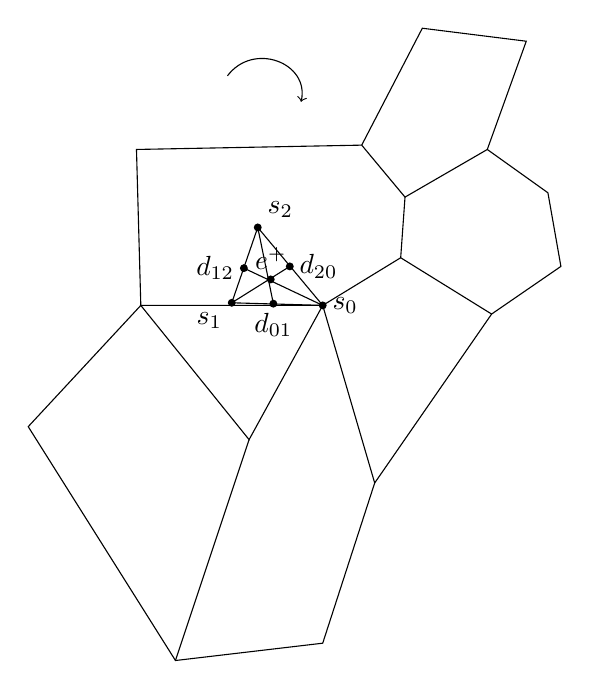
\begin{tikzpicture}[scale=1.1]
\coordinate (a) at (-1.5,0);\coordinate (b) at (.6,0);
\coordinate (c) at (1.5,.55);\coordinate (d) at (1.55,1.25);
\coordinate (e) at (1.05,1.85);\coordinate (f) at (-1.55,1.8);
\draw (a)--(b)--(c)--(d)--(e)--(f)--cycle;
\draw (e)--(1.75,3.2)--(2.95,3.05)--(2.5,1.8)--(d);
\draw (2.5,1.8)--(3.2,1.3)--(3.35,.45)--(2.55,-.1)--(c);
\draw (a)--(-.25,-1.55)--(b)--(1.2,-2.05)--(2.55,-.1);
\draw (a)--(-2.8,-1.4)--(-1.1,-4.1)--(.6,-3.9)--(1.2,-2.05);
\draw (-.25,-1.55)--(-1.1,-4.1);
\draw[->] (-.5,2.65) .. controls (-.2,3.05) and (.45,2.8) .. (.35,2.35);
\coordinate (s1) at (-.45,.03);\coordinate (s2) at (-.15,.9);\coordinate (s0) at (.6,0);
\coordinate (d12) at (-.31,.43);\coordinate (d20) at (.22,.45);\coordinate (d01) at (.03,.02);\coordinate (ep) at (0,.3);
\draw (s1)--(s2)--(s0)--cycle;
\draw (s1)--(d20) (s2)--(d01) (s0)--(d12);
\foreach \p in {s1,s2,s0,d12,d20,d01,ep}{\fill (\p) circle (1.3pt);}
\node[below left] at (s1) {$s_1$};\node[above right] at (s2) {$s_2$};\node[right] at (s0) {$s_0$};
\node[left] at (d12) {$d_{12}$};\node[right] at (d20) {$d_{20}$};\node[below] at (d01) {$d_{01}$};\node[above] at (ep) {$e^+$};
\end{tikzpicture}}

\figure{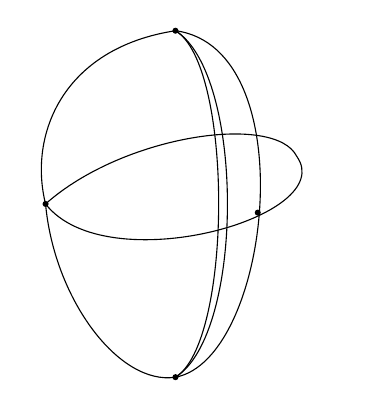
\begin{tikzpicture}[scale=1.1]
\draw (0,2) .. controls (-1.3,1.8) and (-1.7,.8) .. (-1.5,0)
 .. controls (-1.4,-1.1) and (-.65,-2.1) .. (0,-2)
 .. controls (1.1,-1.8) and (1.5,1.8) .. (0,2);
\draw (0,2) .. controls (.8,1.5) and (.8,-1.5) .. (0,-2);
\draw (0,2) .. controls (.67,1.6) and (.66,-1.6) .. (0,-2);
\draw (-1.5,0) .. controls (-.6,.8) and (1.15,1.05) .. (1.4,.55) .. controls (1.9,-.15) and (-.8,-.9) .. (-1.5,0);
\fill (0,2) circle (1pt);\fill (0,-2) circle (1pt);
\fill (-1.5,0) circle (1pt);\fill (.95,-.1) circle (1pt);
\end{tikzpicture}}
\diagram{\begin{tikzcd}[ampersand replacement=\&]
\mathbb P^1_{\overline{\mathbb Q}} \& \mathbb P^1_{\overline{\mathbb Q}}\arrow[l,"\varphi"']
\end{tikzcd}}
\figure{\begin{tikzpicture}[scale=2]
\draw (-1.08,0)--(2.45,0);\draw (.5,-1.4)--(.5,1.8);
\draw (0,0) circle (1);\draw (1,0) circle (1);
\draw[gray,thin] (-1,.02) .. controls (-.95,.9) and (-.2,1.22) .. (.5,.866)
 .. controls (1.15,1.25) and (1.9,.9) .. (2,.02);
\draw[gray,thin] (0,-.03) .. controls (.05,-.7) and (.3,-.86) .. (.5,-.866)
 .. controls (1.1,-1.15) and (1.8,-.9) .. (2,-.03);
\foreach \x in {-1,0,.5,1,2}{\draw (\x,-.025)--(\x,.025);}
\node[below] at (-1,-.03) {$-1$};\node[below] at (0,-.03) {$0$};
\node[below] at (.5,-.03) {$\tfrac12$};\node[below] at (1,-.03) {$1$};\node[below] at (2,-.03) {$2$};
\node[above right] at (.5,.866) {$-j$};
\fill (.5,-.866) circle (.9pt);\node[right] at (.5,-.866) {$-\bar j$};
\end{tikzpicture}}
